\documentclass[border=6pt]{standalone}
\usepackage{tikz}
\usetikzlibrary{arrows.meta,positioning,fit,calc}
\definecolor{fg}{HTML}{000000}
\definecolor{fgbody}{HTML}{000000}
\definecolor{stroke}{HTML}{000000}
\definecolor{surf}{HTML}{F2F2FF}
\definecolor{surfemph}{HTML}{E0E0FF}
\definecolor{surfact}{HTML}{FFEDDB}
\definecolor{bdim}{HTML}{000000}
\definecolor{bemph}{HTML}{000000}
\definecolor{bact}{HTML}{000000}
\begin{document}
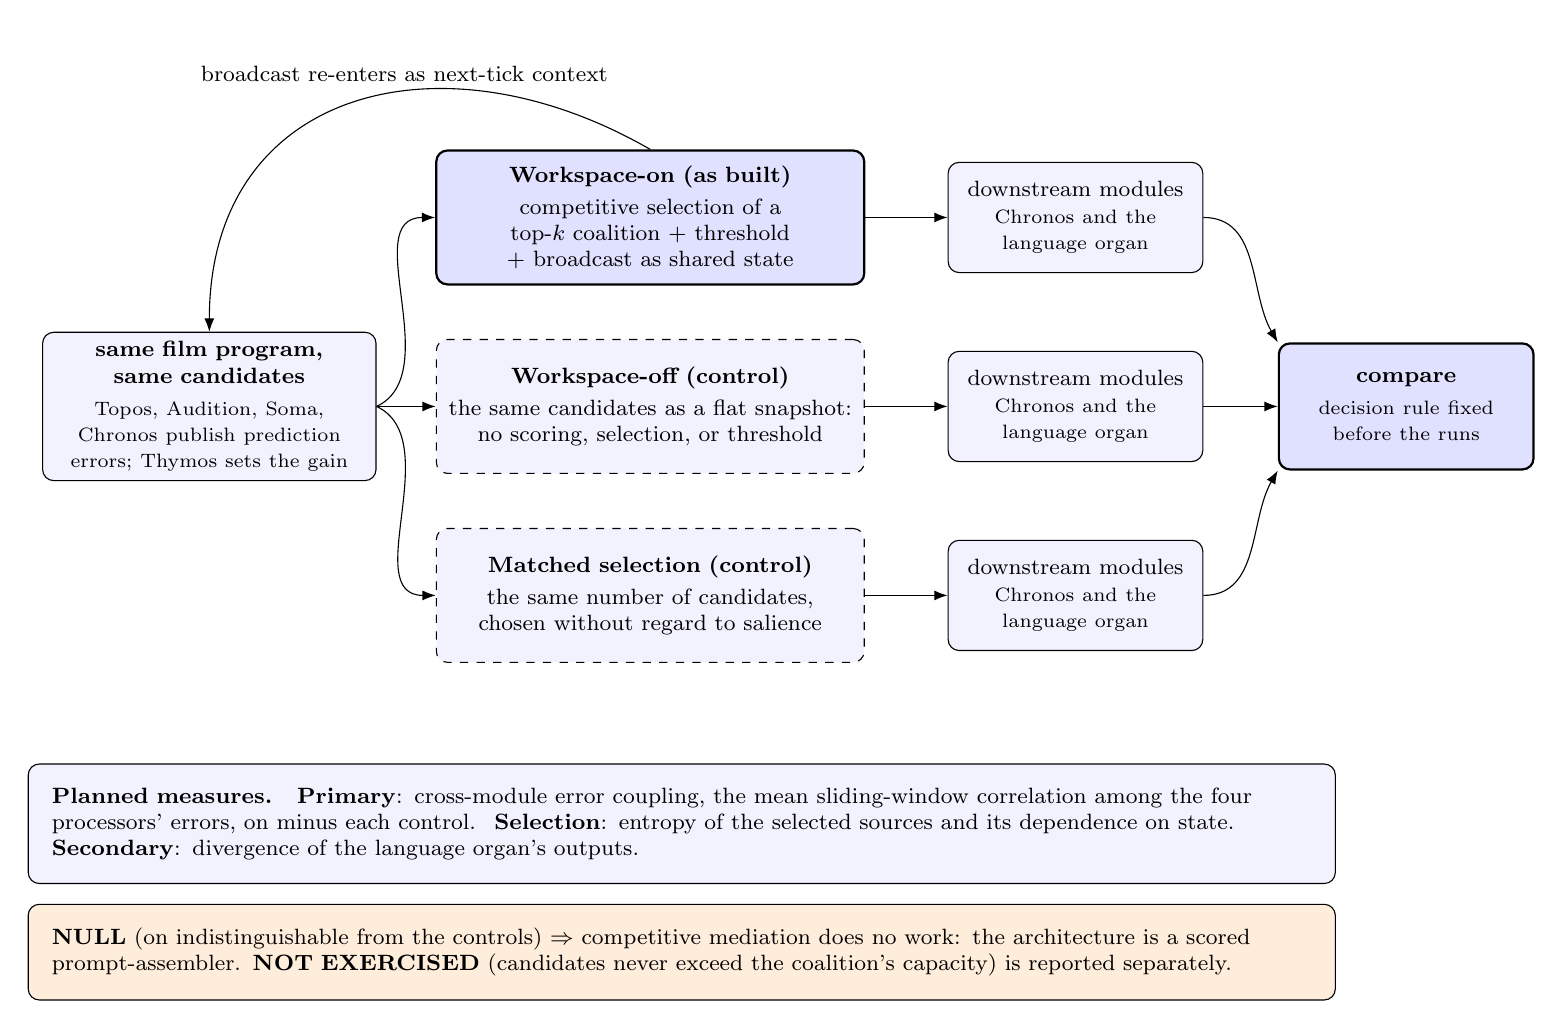
\begin{tikzpicture}[
  font=\small,>=Latex,
  every node/.append style={text=fgbody},
  every node/.append style={execute at begin node={\hyphenpenalty=10000\exhyphenpenalty=10000}},
  mod/.style={draw=bdim, rounded corners, fill=surf, align=center, font=\footnotesize},
  on/.style={draw=bemph, thick, rounded corners, fill=surfemph, align=center, font=\footnotesize},
  off/.style={draw=bdim, dashed, rounded corners, fill=surf, align=center, font=\footnotesize},
  halt/.style={draw=bact, rounded corners, fill=surfact, align=center, font=\footnotesize},
  lbl/.style={font=\footnotesize, text=fgbody, align=center},
]
% shared input
\node[mod, text width=40mm, minimum height=18mm] (shared) at (0,0)
  {\textbf{same film program,\\same candidates}\\[2pt]\scriptsize Topos, Audition, Soma, Chronos publish prediction errors; Thymos sets the gain};
% three arms
\node[on, text width=52mm, minimum height=17mm] (on) at (5.6,2.4)
  {\textcolor{fg}{\textbf{Workspace-on (as built)}}\\[2pt]competitive selection of a \mbox{top-$k$} coalition $+$ threshold $+$ broadcast as shared state};
\node[off, text width=52mm, minimum height=17mm] (off) at (5.6,0)
  {\textcolor{fg}{\textbf{Workspace-off (control)}}\\[2pt]the same candidates as a flat snapshot: no scoring, selection, or threshold};
\node[off, text width=52mm, minimum height=17mm] (match) at (5.6,-2.4)
  {\textcolor{fg}{\textbf{Matched selection (control)}}\\[2pt]the same number of candidates, chosen without regard to salience};
% downstream nodes
\node[mod, text width=30mm, minimum height=14mm] (lon) at (11.0,2.4) {downstream modules\\\scriptsize Chronos and the language organ};
\node[mod, text width=30mm, minimum height=14mm] (loff) at (11.0,0) {downstream modules\\\scriptsize Chronos and the language organ};
\node[mod, text width=30mm, minimum height=14mm] (lmatch) at (11.0,-2.4) {downstream modules\\\scriptsize Chronos and the language organ};
% compare
\node[on, text width=30mm, minimum height=16mm] (cmp) at (15.2,0)
  {\textcolor{fg}{\textbf{compare}}\\[2pt]\scriptsize decision rule fixed before the runs};
% flows
\draw[->, draw=stroke] (shared.east) to[out=25,in=180] (on.west);
\draw[->, draw=stroke] (shared.east) -- (off.west);
\draw[->, draw=stroke] (shared.east) to[out=-25,in=180] (match.west);
\draw[->, draw=stroke] (on) -- (lon);
\draw[->, draw=stroke] (off) -- (loff);
\draw[->, draw=stroke] (match) -- (lmatch);
\draw[->, draw=stroke] (lon.east) to[out=0,in=120] (cmp.north west);
\draw[->, draw=stroke] (loff.east) -- (cmp.west);
\draw[->, draw=stroke] (lmatch.east) to[out=0,in=240] (cmp.south west);
% broadcast re-enters on the on-arm
\draw[->, draw=stroke] (on.north) to[out=150,in=90,looseness=1.3]
  node[lbl, above, pos=0.4]{broadcast re-enters as next-tick context} (shared.north);
% measures + outcome
\node[mod, text width=160mm, align=left, inner sep=3mm] (meas) at (6.0,-5.3)
  {\textbf{Planned measures.}\;\;
   \textbf{Primary}: cross-module error coupling, the mean sliding-window correlation among the four processors' errors, on minus each control.\;
   \textbf{Selection}: entropy of the selected sources and its dependence on state.\;
   \textbf{Secondary}: divergence of the language organ's outputs.};
\node[halt, text width=160mm, align=left, inner sep=3mm, below=2.5mm of meas] (out)
  {\textbf{NULL} (on indistinguishable from the controls) $\Rightarrow$ competitive mediation does no work: the architecture is a scored prompt-assembler. \textbf{NOT EXERCISED} (candidates never exceed the coalition's capacity) is reported separately.};
\end{tikzpicture}
\end{document}
